\chapter*{Report}
\section*{Task 1}
The dataset 5 are picked in this task. 
\begin{figure}[ht]\centering
	\subfigure[Tempereture change]{
		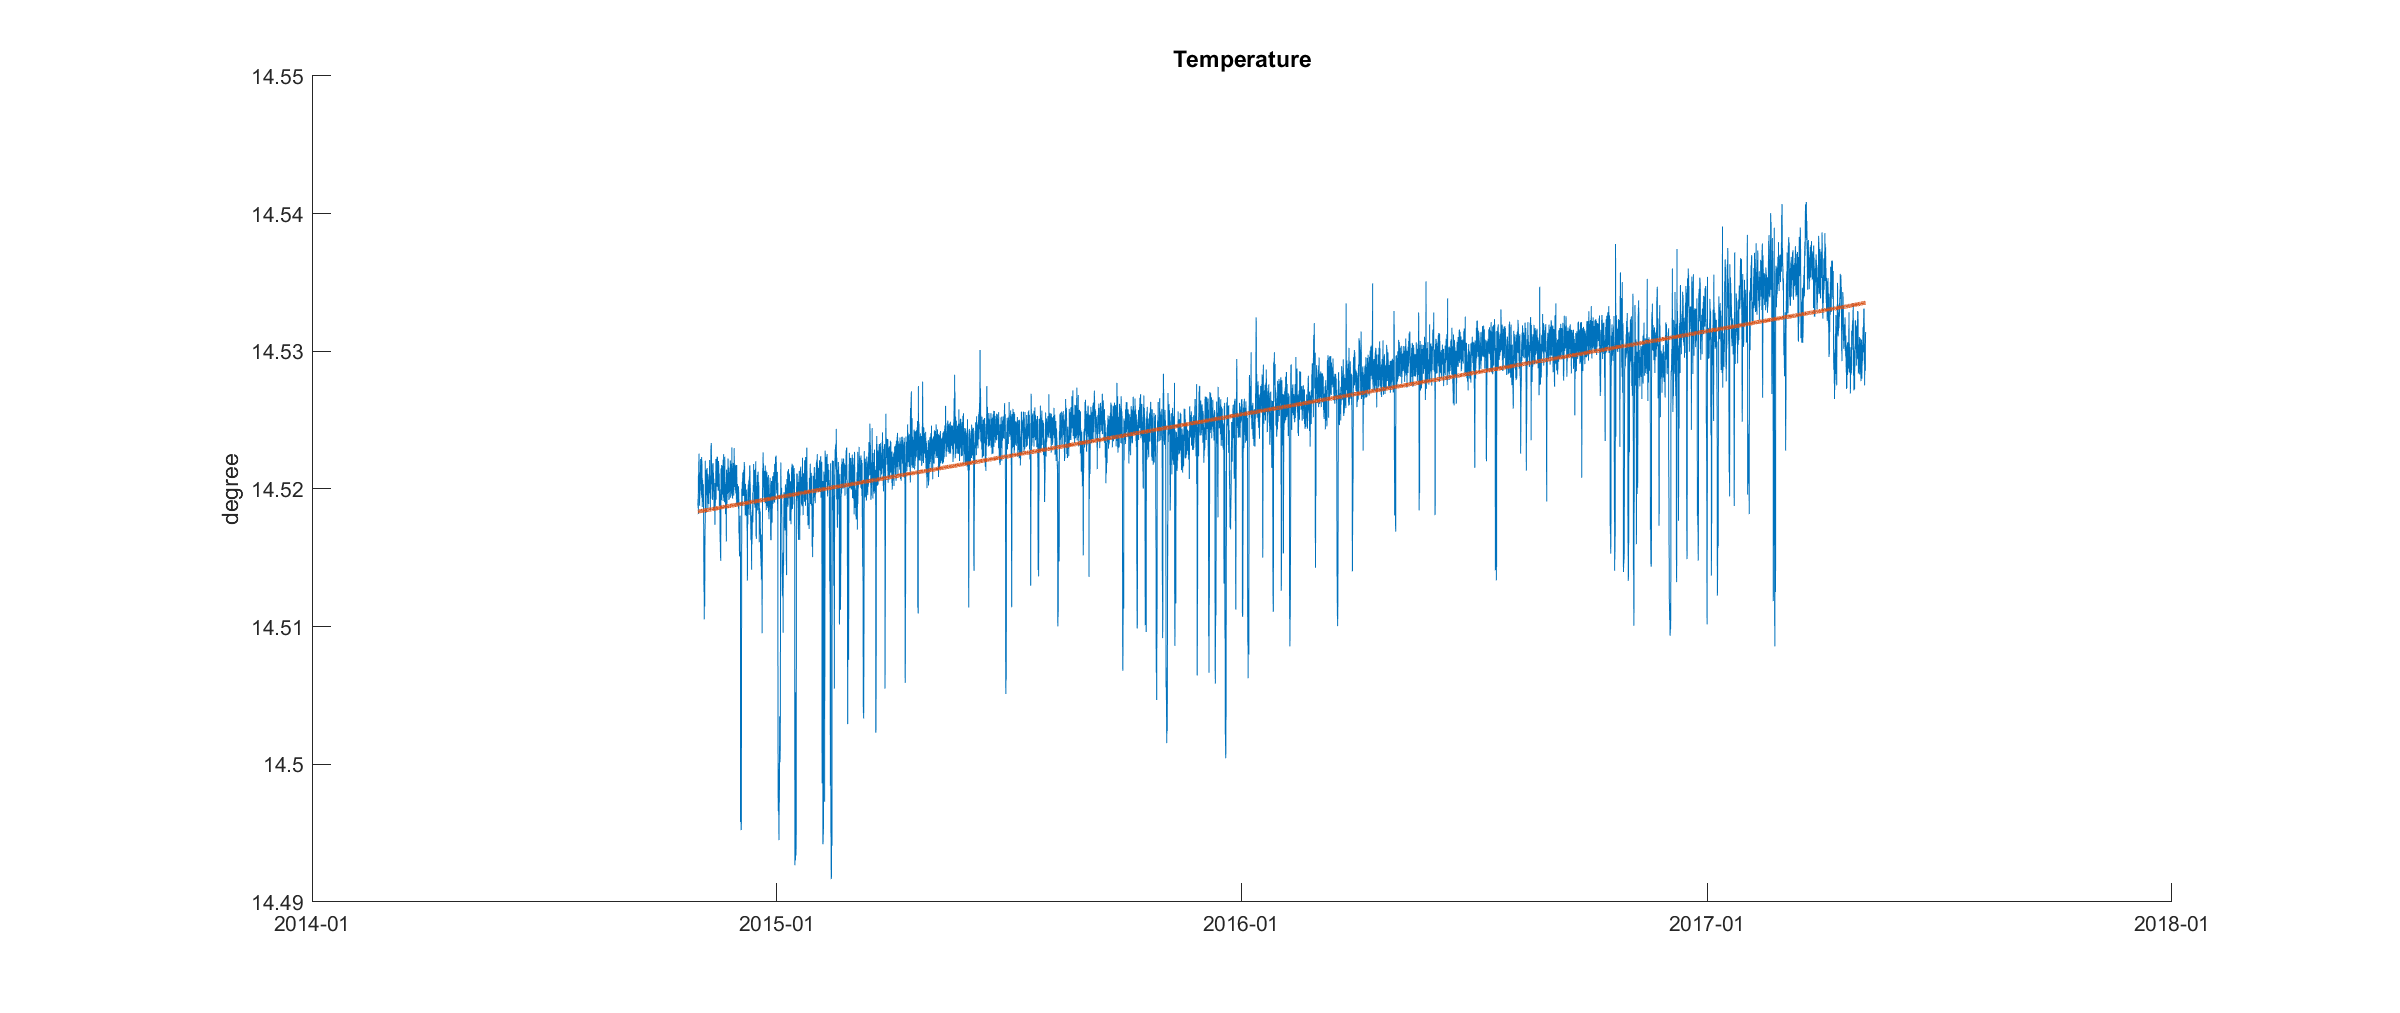
\includegraphics[width=0.9\textwidth]{TempChange.png}}
	\subfigure[Pressure change]{
		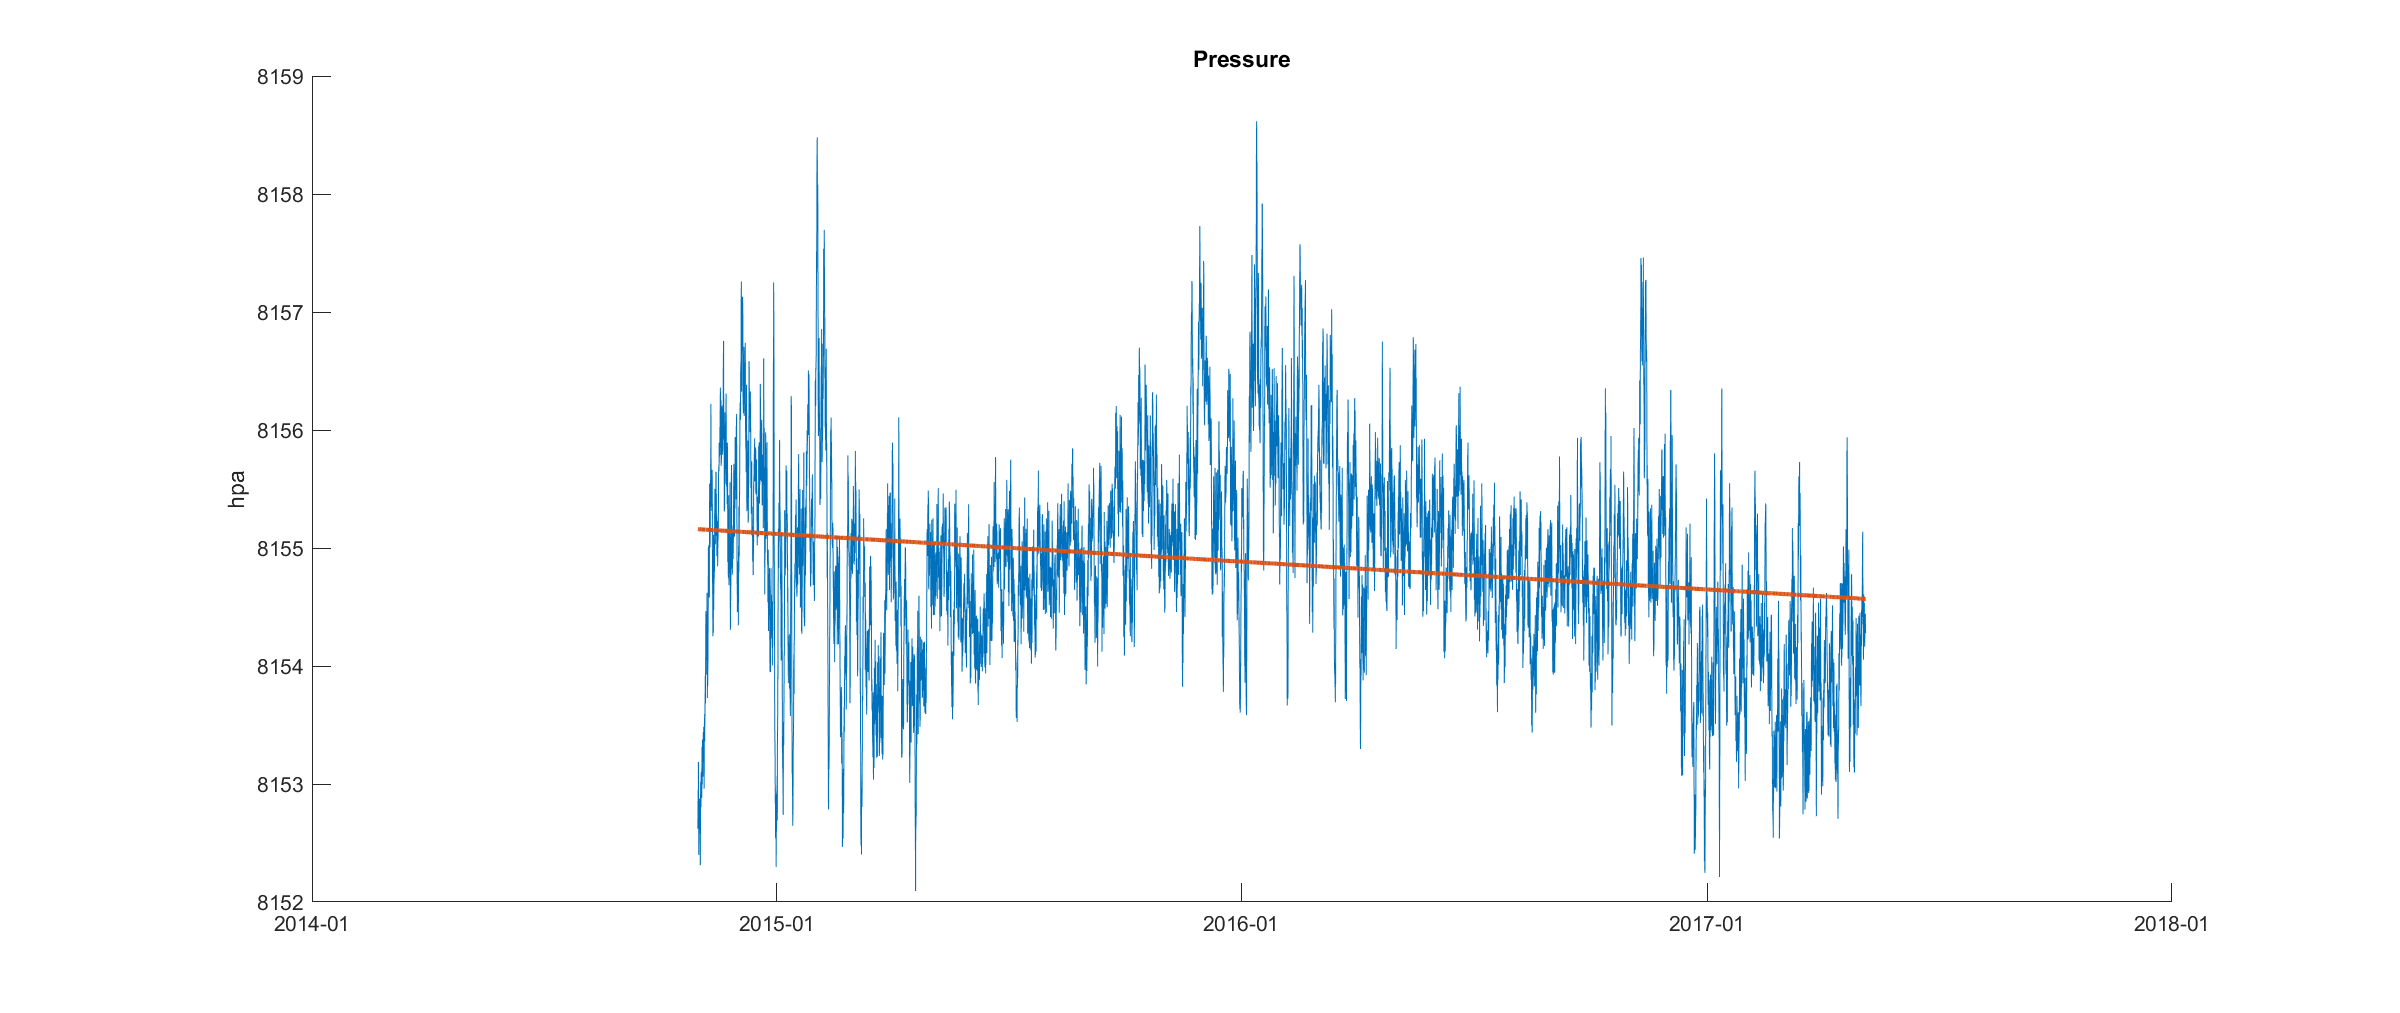
\includegraphics[width=0.9\textwidth]{PressChange.png}}
	\caption{Time series}
\end{figure}
The Temperature and Pressure both have seasonal behavior, in winter the temperature are lower than in summer while the pressure are bigger. The pressure change should come from the density change of the water. \\\\
The temperature has been increased during 2015 to 2017 because of the global warming effect. This also causes the pressure change of the seawater.
\section*{Task 2}
The sw.svel Funktion calculated the sound velocity with the input temperature, salinity and pressure conditions. the T90conv function converts temperature from IPTS48 or IPTS68 to ITS90 standards.\\\\
The influence of these parameters on the sound velocity are in \autoref{fig:soundvelocity}
\begin{figure}[ht]\centering
	\subfigure[Tempereture]{
		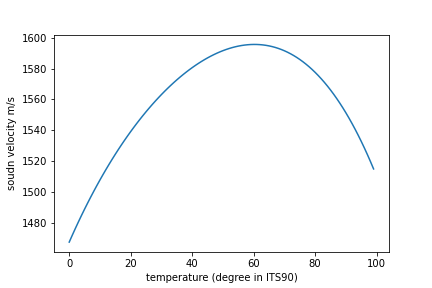
\includegraphics[width=0.45\textwidth]{tempereture.png}}
	\subfigure[Salinity]{
		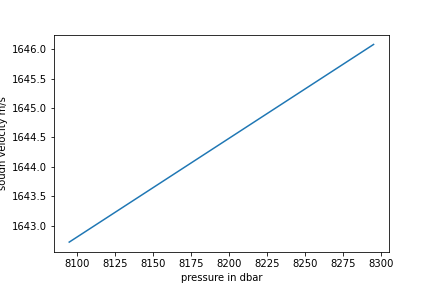
\includegraphics[width=0.45\textwidth]{pressure.png}}
	\subfigure[Pressure]{
		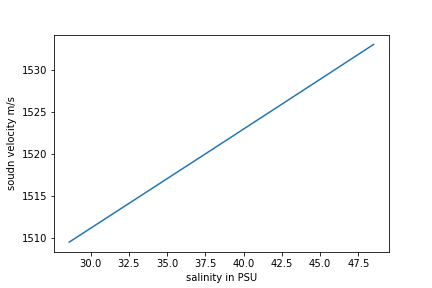
\includegraphics[width=0.45\textwidth]{salinity.png}}
	\caption{Sound velocity change}
	\label{fig:soundvelocity}
\end{figure}\\\\
It was seen that the the sound velocity increases when the salinity and pressure are higher. When the temperature increases, sound velocity gets faster til about 60 $^\circ C$, and then become lower. At this case the temperature is $14 ^\circ C$, where the sound goes faster with higher temperature.
\section*{Task 3}
The gradient are in given code calculated (at $T = 14\ut{^\circ C}$, $s = 0.386 \%$, $p = 819.5 \ut{kpa}$):
\begin{gather*}
	\frac{d v}{d T} = 3.172 \ut{m/(^\circ C\cdot s)} \\ 
	\frac{d v}{d s} = 1.179 \ut{m/(PSU\cdot s)} \\ 
	\frac{d v}{d p} = 1.657 \cdot 10^{-3} \ut{m/(kPa\cdot s)} \\ 
\end{gather*}
Where the sound velocity is $1521.275 \ut{m/s}$\\\\
The influence Temperature to the $dl = 1\ut{cm}$ for $l=1\ut{km}$ baseline 
\begin{gather*}
	dl = t \cdot \frac{d v}{d T} \cdot dT = \frac{l}{v} \cdot \frac{d v}{d T} \cdot dT\\
	dT = dl \cdot \frac{v}{l} \cdot \frac{dT}{dv} = 0.005 \ut{^\circ C}\\
\end{gather*}
Just like above, the influence of salinity and pressure can be calculated: 
\begin{gather*}
	ds = 0.013 \text{\textperthousand} \\
	dp = 9.179 \ut{kpa}
\end{gather*}
\section*{Task 4}
\begin{gather*}
	p_{pasca} = \rho_{water} \cdot g \cdot h_{water} \\
	h_{water} = \frac{p_{pasca}}{\rho_{water} \cdot g}
\end{gather*}
The density of water $\rho_{water}$ and gravity $g$ depend on specific situation. At $T = 4 ^\circ$ is $\rho_{water} = 999.9720 \ut{kg/m^3}$ and if we take $g = 9.80 \ut{m/s^2}$, then:
\begin{equation*}
	h_{water} = \frac{p_{pasca}}{9799.726} \ut{m}
\end{equation*} 